\subsubsection{UART}
\label{subsub:uart}
Die UART Schnittstelle dient der Kommunikation zwischen Raspberry Pi und
dem Freedomboard, welches die LowLevel Funktionalität der Maschine 
umsetzt. Dieses implementiert sämtliche Ansteuerng von Hardwarekomponenten
wie Motorentreibern oder Sensoren. Die übergeordnete Instanz des Freedomboards
ist das Raspberry Pi, welches die Schnittstelle zum Benutzer bildet. Die für
diese Abstraktion notwendige Schnittstelle wird mittels UART
implementiert. UART\footnote{Universal Asynchronous Receiver Transmitter}
ist ein weit verbreiteter Standard für serielle Schnittstellen.  Ein mögliches
Protokoll ist in der Tabelle \ref{tab:uart}
zusammengefasst. Optionale Parameter sind dabei in eckige Klammern gesetzt.
Die erlaubt es einfachere Automaten bzw. Statemachines zu erstellen, da das
setzen und auslesen von Parametern mit den selben Kommandos erfolgt.

Die serielle Schnittstelle wird vom Freedomboard direkt implementiert auf
USB mittels einer USB-Seriell Wandlung. Dies ermöglicht es, das Freedomboard
direkt per USB-Kabel am Raspberry Pi zu verbinden.

\begin{table}[h!]
	\centering
	\begin{tabular}{l l l l l}
		Aktion & Message & Parameter & Antwort \\
		\hline
		drehen um $\varphi$ 
			& \verb!rotate!
			& [Winkel $\varphi$]
			& aktuelle Position \\
		Entfernung $s$ setzen
			& \verb!distance!
			& [Entfernung $s$]
			& aktuelle Entfernung \\
		Ausrichtungsmotor enable
			& \verb!rotater!
			& [enable/disable]
			& aktueller Status \\
		Schussmotor enable
			& \verb!shooter! 
			& [enable/disable]
			& aktueller Status \\
		Lademotor enable
			& \verb!loader!
			& [enable/disable]
			& aktueller Status \\
		Schussmotor einstellen
			& \verb!setrpm!
			& [RPM]
			& aktueller Status \\
		Schussabgabe
			& \verb!fire!
			& -
			& ok/nok \\
		Reset
			& \verb!reset!
			& -
			& -\\
	\end{tabular}
	\caption{Protokollentwurf der seriellen Schnittstelle}
	\label{tab:uart}
\end{table}

Für die Entwicklungsphase sind zu den in der Tabelle \ref{tab:uart}
aufgeführten Kommandos noch weitere zu implementieren. Beispielsweise
ist es nützlich, einige Maxima und Minima für allfällige
Reglerparametrierungen abrufen zu können. Ein Besipiel hierfür ist das
Anfahren und Zurückstellen des Schussmotors wie in der Abbildung
\ref{fig:shooter} dargestellt.

\begin{comment}
\begin{figure}[h!]
	\centering
	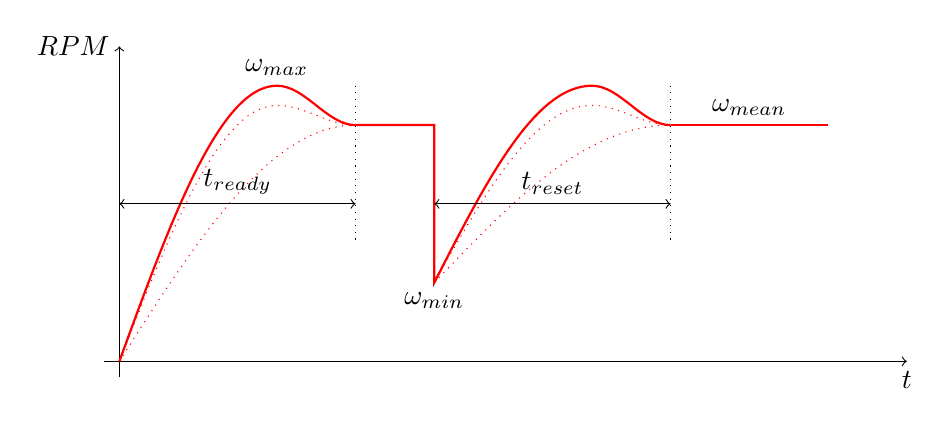
\begin{tikzpicture}
		% Koordinaten
		\draw[->] (-0.2,0) -- (10,0) node[anchor=north] {$t$};
		\draw[->] (0,-0.2) -- (0,4) node[anchor=east] {$RPM$};
		% Hilfslinien
		\draw[dotted] (3,3.5) -- (3,1.5);
		\draw[dotted] (7,3.5) -- (7,1.5);
		% Kurve - Anfahren
		\draw[red, thick] 
			(0,0) sin (2,3.5) cos (2.5,3.25) sin (3,3);
		\draw[red, dotted]
			(0,0) sin (2,3.25) cos (2.5,3.125) sin (3,3);
		\draw[red, dotted]
			(0,0) sin (3,3);
		% Kurve - Einbruch
		\draw[red, thick] 
			(3,3) -- (4,3) -- 
			(4,1) sin (6,3.5) cos (6.5,3.25) sin (7,3);
		\draw[red, dotted]
			(4,1) sin (6,3.25) cos (6.5,3.125) sin (7,3);
		\draw[red, dotted]
			(4,1) sin (7,3);
		% Kurve - Ende
		\draw[red, thick] (7,3) -- (9,3);
		% Markierungen
		\draw[] (2,3.5) node[anchor=south] {$\omega_{max}$};
		\draw[] (4,1) node[anchor=north] {$\omega_{min}$};
		%\draw[] (4,3) node[anchor=south] {Schuss};
		\draw[] (8,3) node[anchor=south] {$\omega_{mean}$};
		% Zeiten
		\draw[<->] (0,2) -- (3,2) node[midway, above] {$t_{ready}$};
		\draw[<->] (4,2) -- (7,2) node[midway, above] {$t_{reset}$};
	\end{tikzpicture}
	\caption{Vereinfachter Verlauf der Schussmotorendrehzahl für Anfahrt
		und einfache Schussabgabe}
	\label{fig:shooter}
\end{figure}
\end{comment}

\begin{figure}[h!]
	\centering
	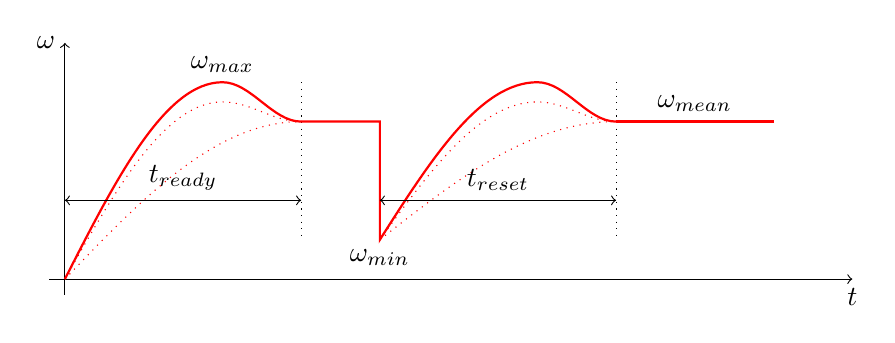
\begin{tikzpicture}
		% Koordinaten
		\draw[->] (-0.2,0) -- (10,0) node[anchor=north] {$t$};
		\draw[->] (0,-0.2) -- (0,3) node[anchor=east] {$\omega$};
		% Hilfslinien
		\draw[dotted] (3,2.5) -- (3,0.5);
		\draw[dotted] (7,2.5) -- (7,0.5);
		% Kurve - Anfahren
		\draw[red, thick] 
			(0,0) sin (2,2.5) cos (2.5,2.25) sin (3,2);
		\draw[red, dotted]
			(0,0) sin (2,2.25) cos (2.5,2.125) sin (3,2);
		\draw[red, dotted]
			(0,0) sin (3,2);
		% Kurve - Einbruch
		\draw[red, thick] 
			(3,2) -- (4,2) -- 
			(4,0.5) sin (6,2.5) cos (6.5,2.25) sin (7,2);
		\draw[red, dotted]
			(4,0.5) sin (6,2.25) cos (6.5,2.125) sin (7,2);
		\draw[red, dotted]
			(4,0.5) sin (7,2);
		% Kurve - Ende
		\draw[red, thick] (7,2) -- (9,2);
		% Markierungen
		\draw[] (2,2.5) node[anchor=south] {$\omega_{max}$};
		\draw[] (4,0.5) node[anchor=north] {$\omega_{min}$};
		%\draw[] (4,3) node[anchor=south] {Schuss};
		\draw[] (8,2) node[anchor=south] {$\omega_{mean}$};
		% Zeiten
		\draw[<->] (0,1) -- (3,1) node[midway, above] {$t_{ready}$};
		\draw[<->] (4,1) -- (7,1) node[midway, above] {$t_{reset}$};
	\end{tikzpicture}
	\caption{Vereinfachter Verlauf der Schussmotorendrehzahl für Anfahrt
		und einfache Schussabgabe}
	\label{fig:shooter}
\end{figure}
